\documentclass[]{article}

\usepackage{fancyhdr}
 \pagestyle{fancy}
\rhead{\textsc{Scott O`Connor}}

\usepackage{lmodern}
\usepackage{amssymb,amsmath}
\usepackage{ifxetex,ifluatex}
\usepackage{fixltx2e} % provides \textsubscript
\ifnum 0\ifxetex 1\fi\ifluatex 1\fi=0 % if pdftex
  \usepackage[T1]{fontenc}
  \usepackage[utf8]{inputenc}
\else % if luatex or xelatex
  \ifxetex
    \usepackage{mathspec}
    \usepackage{xltxtra,xunicode}
  \else
    \usepackage{fontspec}
  \fi
  \defaultfontfeatures{Mapping=tex-text,Scale=MatchLowercase}
  \newcommand{\euro}{€}
\fi
% use upquote if available, for straight quotes in verbatim environments
\IfFileExists{upquote.sty}{\usepackage{upquote}}{}
% use microtype if available
\IfFileExists{microtype.sty}{%
\usepackage{microtype}
\UseMicrotypeSet[protrusion]{basicmath} % disable protrusion for tt fonts
}{}
\ifxetex
  \usepackage[setpagesize=false, % page size defined by xetex
              unicode=false, % unicode breaks when used with xetex
              xetex]{hyperref}
\else
  \usepackage[unicode=true]{hyperref}
\fi
\usepackage[usenames,dvipsnames]{color}
\hypersetup{breaklinks=true,
            bookmarks=true,
            pdfauthor={},
            pdftitle={The Meaning of Life},
            colorlinks=true,
            citecolor=blue,
            urlcolor=blue,
            linkcolor=magenta,
            pdfborder={0 0 0}}
\urlstyle{same}  % don't use monospace font for urls
\usepackage{graphicx,grffile}
\makeatletter
\def\maxwidth{\ifdim\Gin@nat@width>\linewidth\linewidth\else\Gin@nat@width\fi}
\def\maxheight{\ifdim\Gin@nat@height>\textheight\textheight\else\Gin@nat@height\fi}
\makeatother
% Scale images if necessary, so that they will not overflow the page
% margins by default, and it is still possible to overwrite the defaults
% using explicit options in \includegraphics[width, height, ...]{}
\setkeys{Gin}{width=\maxwidth,height=\maxheight,keepaspectratio}
\setlength{\parindent}{0pt}
\setlength{\parskip}{6pt plus 2pt minus 1pt}
\setlength{\emergencystretch}{3em}  % prevent overfull lines
\providecommand{\tightlist}{%
  \setlength{\itemsep}{0pt}\setlength{\parskip}{0pt}}
\setcounter{secnumdepth}{0}

\title{The Meaning of Life}
\author{Scott O’Connor}


% Redefines (sub)paragraphs to behave more like sections
\ifx\paragraph\undefined\else
\let\oldparagraph\paragraph
\renewcommand{\paragraph}[1]{\oldparagraph{#1}\mbox{}}
\fi
\ifx\subparagraph\undefined\else
\let\oldsubparagraph\subparagraph
\renewcommand{\subparagraph}[1]{\oldsubparagraph{#1}\mbox{}}
\fi

\begin{document}
\maketitle

\section{The Meaning of Life}\label{the-meaning-of-life}

\subsection{Personal Note}\label{personal-note}

We will be talking about death, suicide, and depression in this module.
These are uncomfortable topics for many and have touched most of us
directly or indirectly. They raise core philosophical questions, perhaps
raise the most important philosophical questions. I would like to
encourage you to keep a very open mind about the material. Don't accept
that, say, you are better off being dead only after reading the material
for a few days. A full and proper study of the issues would take many
years. You might also like to know that NJCU offers
\href{http://www.njcu.edu/counselingcenter}{free counseling services} to
registered NJCU students.

\subsection{Introduction}\label{introduction}

You are mortal. Your friends, families, and loved ones are mortal. Each
of us will die. It is easy to ignore it. We often think of death as
happening some point in the far future. Like a distant land that we may
have to visit one day, that land is not this land and we are happy to
ignore it. Unfortunately, death is an ever pressing possibility. Several
have recently died from Legionnaires disease in the Bronx. Many are
killed in car accidents every day. There are the bizarre accidents too.
Walking to work you don't think that this might be the day you die. It's
too depressing! But you could die at any moment. You might stumble and
hit your head awkwardly. A wall might collapse upon you.

In this module, we are going to examine Leo Tolstoy's argument that our
mortality robs our life of meaning, though, we will also look at the
meaning he did finally find in life. Tolstoy puts his concern as
follows:

\begin{quote}
\ldots{} My question - that which at the age of fifty brought me to the
verge of suicide - was the simplest of questions, lying in the soul of
every man from the foolish child to the wisest elder: it was a question
without an answer to which one cannot live, as I had found by
experience. It was: ``What will come of what I am doing today or shall
do tomorrow? What will come of my whole life?''
\end{quote}

\begin{quote}
Differently expressed, the question is: ``Why should I live, why wish
for anything, or do anything?'' It can also be expressed thus: ``Is
there any meaning in my life that the inevitable death awaiting me does
not destroy?''\ldots{}
\end{quote}

This handout proceeds in the three parts. The first clarifies the
question that concerns Tolstoy. The second part explains his initial
argument that life has no meaning. The third discusses his subsequent
claim to have found the meaning of life in faith, in the Russian
Orthodox Church.

\subsubsection{Clarifying the Question.}\label{clarifying-the-question.}

The question that concerns us, `what's the meaning of life?' seems a
good one. It's certainly one you can imagine anyone, philosopher or not,
raising and trying to answer. However, the question is itself misleading
and any hope of answering it will require that we identify what exactly
it is asking.

Why is it misleading? `Meaning' is a property of words and phrases. You
can ask about the meaning of, say, the word `cacophony', but you cannot
ask about the meaning of, say, the sun. The sun is a physical entity.
Physical entities do not have meanings at all.

When we ask after the meaning of life, we are not concerned with the
meaning of the word `life'. Answering the question would then just
require us to consult the relevant entry in a dictionary. We are asking
something deeper, something about why we should live at all. The
question arises, on the one hand, because we find ourselves on this
Earth alive, living a life, having never chosen to in fact be alive. On
the other hand, we find ourselves with lives that can be ended at any
moment we choose. We would like to know why we should prefer to continue
with life rather than to end it all.

Similarly, suppose you wake up at a party after being knocked out and
brought there without your input. You can leave the party at any time.
It's completely up to you. If you stay, you should have a reason for
staying. Might you be better off leaving? Similarly, none of us have
chosen to live, but we can all end our lives at any moment. If we choose
not to leave, not to end our lives, we should have a reason for our
choice. Why is living better than dying?

Understood in this way, life has meaning only if it has significant
value or purpose over time, where this value makes life choice worthy.
There are two different ways of understanding this value:

\begin{itemize}
\item
  \textbf{Internal Value:} the value or purpose that comes when people
  see their goals or purposes as inherently valuable or worthwhile.
\item
  \textbf{External Value:} Meaning or purpose that comes from outside of
  ourselves in relationship to something that we may or may not be aware
  of.
\end{itemize}

Let us illustrate the difference with an example. What value does the
life of a bee have? From an external point of view, it has value to bee
keepers and honey eaters. For the former, bees are significant for their
career. For the latter, bees are significant for their nourishment. From
an internal point of view, a bee's life would have meaning if a bee
could come to see one of its projects as worthwhile, if it come to value
some project. So, for instance, if a worker bee could come to see the
project of serving the queen as worthwhile, the bee would find value in
its life.

When we ask about the meaning of life, we are asking about internal
value. We are asking why we should feel that there is something in our
lives that make them worthwhile. Is there any project or goal that could
make our lives choice worthy, could shape our psychology so dramatically
that we are motivated to get up in the morning, keep going, and find all
the trials and tribulations of life worthwhile?

We will see that Tolstoy initially believes that nothing can play this
role, nothing could give life internal value. His argument relies on the
assumption that life will only have internal value, it will be something
that we can find choice worthy, if life has external value. Tolstoy
initially thinks that death undermines any external meaning our lives
might have. Our lives last a mere moment from the perspective of the
universe. Even if our accomplishments outlive us, they too will one day
be forgotten. We cannot even say that we live for our family; they will
die in no time at all from the perspective of the universe.

\subsection{Pessimism}\label{pessimism}

Pessimism is the view that life has no meaning at all. The argument for
it is straightforward:

\begin{enumerate}
\def\labelenumi{\arabic{enumi}.}
\tightlist
\item
  Life is choice worthy only if it has internal value.
\item
  Life has internal value only if life has external value.
\item
  Life has no external value.
\item
  Life has no internal value.
\item
  Life is not choice worthy.
\end{enumerate}

The two key premises are 2 and 3. Distinguish the question whether life
is valuable from the question whether things like education, health,
eradicating world hunger, writing a great novel, family, and so on.
These latter things are candidates for the goals and projects that we
might find as valuable and so give to our lives internal value. Premise
2 says that any of these candidates can give life internal value only if
they, themselves, have external value. Premise 3 says that no candidate
does, in fact, have external value. Tolstoy argues for Premise 3 by way
of a fable:

\begin{figure}[htbp]
\centering
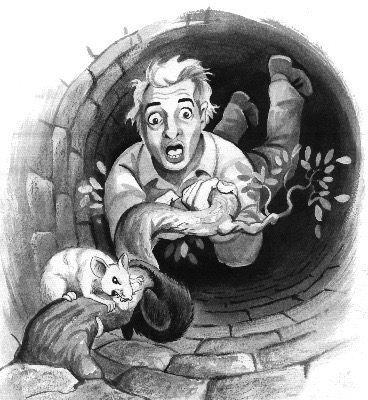
\includegraphics{Tolstoy.jpg}
\caption{alt text}
\end{figure}

\begin{quote}
Imagine a traveller fleeing a ferocious, hungry beast. Our traveller's
only means of escape is a well they stumble upon. They jump down to
escape the infuriated beast who remains waiting at the well's edge. Some
great trees grow beside our well, its roots jutting down and through its
walls. The traveller reaches out, grabs the roots and saves himself from
falling, which turns out quite fortuitous for him. As his eyes adjust,
the traveller notices red glowing eyes at the bottom of the well. A
dragon!
\end{quote}

\begin{quote}
Our traveler is stuck. The beast above awaits if he climbs up. The
dragon below awaits if he climbs down. He pauses, clutching the roots
growing from the cleft of the well wall. Things get worse. Two mice, one
black and one white, appear and start nibbling on the roots. Our
traveller realizes that the roots will break and inevitably he will fall
into the dragon's jaws below.
\end{quote}

\begin{quote}
While he is still clinging, he sees some drops of honey hanging on the
roots, and so reaches out for them with his tongue. He tastes the
sweetness, which distracts him for a while from the beast above, the
dragon below, and the mice eating the roots.
\end{quote}

This fable, says Tolstoy, depicts the life each of us live. The dragon
and beast represent death. The mice represent time. The honey represents
those things we use to distract ourselves from our mortality, family,
career, etc. These are supposed to be what give our lives internal
value, they are the things that make us think that life is choice
worthy. But would you find the honey sweet if you were in that well?
Maybe initially. But your awareness of the dragon, beast, and mice will
likely dampen, if not destroy, your continued enjoyment of the honey.
Similarly, Tolstoy suggests that none of the things we use to distract
ourselves from our mortality can continue to do so indefinitely. He
claims:

\begin{quote}
``Just so I hold on to the branch of life, knowing that the dragon of
death is waiting inevitably for me, ready to tear me to pieces, and I
cannot understand why I have fallen on such suffering. And I try to lick
that honey which used to give me pleasure, but now it no longer gives me
joy, and the white and black mouse day and night nibble at the branch to
which I am holding on. I clearly see the dragon, and the honey is no
longer sweet to me. I see only the inevitable dragon and the mice, and
am unable to turn my glance away from them. This is not a fable, but a
veritable, indisputable, comprehensible truth.''
\end{quote}

\begin{quote}
`'The deception of the joys of life which formerly allayed my terror of
the dragon now no longer deceived me\ldots{}The two drops of honey which
diverted my eyes from the cruel truth longer than the rest: my love of
family, and of writing - art as I called it - were no longer sweet to
me.''
\end{quote}

\begin{quote}
``Family''\ldots{}said I to myself. But my family - wife and children -
are also human. They are placed just as I am: they must either live in a
lie or see the terrible truth. Why should they live? Why should I love
them, guard them, bring them up, or watch them? That they may come to
the despair that I feel, or else be stupid? Loving them, I cannot hide
the truth from them: each step in knowledge leads them to the truth. And
the truth is death\ldots{}.No sweetness of honey could be sweet to me
when I saw the dragon and saw the mice gnawing away my support.
\end{quote}

\begin{quote}
It was indeed terrible. And to rid myself of the terror I wished to kill
myself. \ldots{}
\end{quote}

\subsection{Four Attitudes Toward
Death}\label{four-attitudes-toward-death}

If Tolstoy's diagnosis of our lives is correct, there are four attitudes
we can take towards our lives. Similarly, there are four attitudes you
could take while you cling to the well wall:

\begin{enumerate}
\def\labelenumi{\arabic{enumi}.}
\item
  Ignorance: It consists in not knowing, not understanding, that life is
  an evil and an absurdity. People of this sort have yet to see the
  dragon that awaits them. They have yet to see the mice gnawing the
  shrub by which they are hanging. The lick the honey. They do so only
  for a while: something will eventually turn their attention to the
  dragon and the mice. They will then stop their licking.
\item
  Epicureanism: while knowing the hopelessness of life, make use
  meanwhile of the advantages one has, disregarding the dragon and the
  mice, and licking the honey in the best way, especially if there is
  much of it within reach. This, though, is an unsustainable attitude.
  Many live in terrible conditions. Many have no honey to taste. It is a
  mere accident, claims Tolstoy, that you have good circumstances rather
  than poor, and `'the accident that has today made me a Solomon may
  tomorrow make me a Solomon's slave.'' Epicureans try but cannot
  ultimately forget that all these pleasures are ephemeral. They are as
  easily lost as gained. Nobody can be confident that life will always
  provide these distractions.
\item
  Weakness: ``It consists in seeing the truth of the situation and yet
  clinging to life, knowing in advance that nothing can come of it.
  People of this kind know that death is better than life, but not
  having the strength to act rationally - to end the deception quickly
  and kill themselves - they seem to wait for something. This is the
  escape of weakness, for if I know what is best and it is within my
  power, why not yield to what is best?''
\item
  Suicide: ``This is the way of strength and energy. It consists in
  destroying life, when one has understood that it is an evil and an
  absurdity. A few exceptionally strong and consistent people act so.
  Having understood the stupidity of the joke that has been played on
  them, and having understood that it is better to be dead than to be
  alive, and that it is best of all not to exist, they act accordingly
  and promptly end this stupid joke.''
\end{enumerate}

\subsection{Optimism}\label{optimism}

Optimists claim that life does have meaning; it does have internal
value. There are two versions of optimism. The first agrees that life
has internal value only if it has external value, but identifies an
external value to life in religion. The second accepts that life has no
external value, but denies that internal value depends on there being
external value. The first is associated with Theism. The second with
Atheism. You can find further discussion of each in the textbook. I
provide a few extra details about the first here.

\subsection{Theism}\label{theism}

Tolstoy did not remain depressed. He reports meeting and talking with
rural farmers at a time in Russia when farmers lived a menial existence.
They had nothing. Yet Tolstoy sees in these rural farmers an acceptance
of life's vicissitudes. Reclaiming his faith, he realized that he had
found value in the wrong things. His art, his family, etc., could never
provide the meaning he had sought. But God, an eternal perfect being,
could provide that value. Tolstoy comes to accept the following two
claims:

\begin{enumerate}
\def\labelenumi{\arabic{enumi}.}
\item
  A human's life has external meaning only because it is part of God's
  plan, a grand cosmic order that encompasses every entity in the
  universe.
\item
  A human's life can have internal meaning if they align their
  life---their goals, projects, ambitions---with God's plan. That is,
  life will be choice worthy if you can identify God's plan for you and
  set about realizing that plan.
\end{enumerate}

\subsection{Meaning \& Christianity}\label{meaning-christianity}

Tolstoy doesn't detail how Christianity construes the meaning of life.
He merely says that if you believe that God exists, then you can see
that your life has some external value. But can we say something more
about what this external value consists in?

At this point, Christians point to one person who, they claim, had a
meaningful life. Jesus's live shows us that God cares about human lives;
Jesus was sent to save mankind. Reflecting on the details of his life,
we might say that Jesus's life had the following meaning:

\textbf{Teleological Value:} His life had a purpose. All of Jesus' life
involves suffering for the sake of man kind. All the aspects of his life
were organized around this one overarching purpose.

Christianity also emphasizes other characters with God given purposes.
Noah, the Saints, the Apostles, are all individuals who were supposedly
given important jobs by God. These tasks, these jobs, give their life
external value according to Christianity. Their lives also had internal
value because they identified their God given purposes, saw them as
worthwhile, and devoted their time and energy to realizing them.

\subsection{Objection}\label{objection}

Here I briefly raise a problem for this account of the meaning of life.
Suppose we grant that the lives of Jesus, Noah, the other Saints had
external value because each of them had a God given purpose. It does not
thereby follow that each human has a God given purpose and some of the
candidates for this purpose are unsatisfactory:

\textbf{Suggestions 1:} Our purpose is to serve God. This is a very
natural suggestion. A Theist might claim that we were created by God to
do his will. That would seem to give our lives the significance we
desired. The problem, though, is that being in service to someone is not
obviously a thing we would always choose. Granted, if God created us to
serve him, then our lives would be significant to God. But notice that
bees are significant to the bee keeper, yet that hardly shows us why a
bee should find its own life significant.

To motivate this objection, consider the very far fetched idea that God
created us to perform a very specific role. Once our species has grown
large enough, he will signal to an alien race to move to Earth where
they will now find a new rich food source. Us! If this were the case,
God would have crated us to be the food in some alien's hamburger. We
would have a role in his grand design. We would even know what it is. I
doubt, though, that anyone would be happy to find out that they were
created as food for some superior being. A menial role in a stage
designed for another does not make life choice worthy.

There is a second worry with the claim that God created us to serve him.
Recall that God is all loving, all knowing, and all powerful. If he is
all loving, he would never have created us merely to serve him,
especially since our lives involve so much suffering and pain. Suppose
that we had the ability to create a a new fully conscious species. It is
only an evil creator that would create such beings to suffer and toil in
servitude to them.

\textbf{Suggestion 2:} The existence of God shows that we have a
purpose. He is all loving, therefore he would never have created us
without a purpose. However, since he is all loving, he would never have
created us merely to serve him. Nevertheless, we do not know why he
created us, to what end he intended our lives to serve.

The suggestion merely avoids answering the question at hand. How, if at
all, would the existence of God provide life with external meaning?

By themselves, these objections do not completely undermine the Theist's
account of the meaning of life. What they do, however, is show that
belief in God should not in itself be comforting. For God's existence to
be comforting, we need to know why he created us, to what end our lives
serve. Unless those details are forthcoming, the unsettling possibility
is left open that he created us for reasons that none of us should be
happy to live with.

\end{document}
